% !TEX TS-program = XeLaTeX
% use the following command:
% all document files must be coded in UTF-8
\documentclass[portuguese]{textolivre}
% build HTML with: make4ht -e build.lua -c textolivre.cfg -x -u article "fn-in,svg,pic-align"

\journalname{Texto Livre}
\thevolume{17}
%\thenumber{1} % old template
\theyear{2024}
\receiveddate{\DTMdisplaydate{2023}{8}{24}{-1}} % YYYY MM DD
\accepteddate{\DTMdisplaydate{2023}{10}{5}{-1}}
\publisheddate{\DTMdisplaydate{2023}{11}{29}{-1}}
\corrauthor{Antonio Marcio da Silva}
\articledoi{10.1590/1983-3652.2024.47836}
%\articleid{NNNN} % if the article ID is not the last 5 numbers of its DOI, provide it using \articleid{} commmand 
% list of available sesscions in the journal: articles, dossier, reports, essays, reviews, interviews, editorial
\articlesessionname{dossier}
\runningauthor{Da Silva e Rottava} 
%\editorname{Leonardo Araújo} % old template
\sectioneditorname{Daniervelin Pereira}
\layouteditorname{Leonado Araújo}

\title{Densidade lexical em textos gerados pelo ChatGPT: implicações da inteligência artificial para a escrita em línguas adicionais}
\othertitle{Lexical density in texts generated by ChatGPT: implications of artificial intelligence for writing in additional languages}
% if there is a third language title, add here:
%\othertitle{Artikelvorlage zur Einreichung beim Texto Livre Journal}

\author[1]{Antonio Marcio Da Silva~\orcid{0000-0002-4628-4091}\thanks{Email: \href{mailto:antonio.dasilva@essex.ac.uk}{antonio.dasilva@essex.ac.uk}}}
\author[2]{Lucia Rottava~\orcid{0000-0003-3094-6270}\thanks{Email: \href{mailto:luciarottava@yahoo.com.br}{luciarottava@yahoo.com.br}}}
\affil[1]{University of Essex, Colchester, Inglaterra.}
\affil[2]{Universidade Federal do Rio Grande do Sul, Instituto de Letras, Porto Alegre, RS, Brasil.}

\addbibresource{article.bib}
% use biber instead of bibtex
% $ biber article

% used to create dummy text for the template file
\definecolor{dark-gray}{gray}{0.35} % color used to display dummy texts
\usepackage{lipsum}
\SetLipsumParListSurrounders{\colorlet{oldcolor}{.}\color{dark-gray}}{\color{oldcolor}}

% used here only to provide the XeLaTeX and BibTeX logos
\usepackage{hologo}

% if you use multirows in a table, include the multirow package
\usepackage{multirow}

% provides sidewaysfigure environment
\usepackage{rotating}

% CUSTOM EPIGRAPH - BEGIN 
%%% https://tex.stackexchange.com/questions/193178/specific-epigraph-style
\usepackage{epigraph}
\renewcommand\textflush{flushright}
\makeatletter
\newlength\epitextskip
\pretocmd{\@epitext}{\em}{}{}
\apptocmd{\@epitext}{\em}{}{}
\patchcmd{\epigraph}{\@epitext{#1}\\}{\@epitext{#1}\\[\epitextskip]}{}{}
\makeatother
\setlength\epigraphrule{0pt}
\setlength\epitextskip{0.5ex}
\setlength\epigraphwidth{.7\textwidth}
% CUSTOM EPIGRAPH - END

% LANGUAGE - BEGIN
% ARABIC
% for languages that use special fonts, you must provide the typeface that will be used
% \setotherlanguage{arabic}
% \newfontfamily\arabicfont[Script=Arabic]{Amiri}
% \newfontfamily\arabicfontsf[Script=Arabic]{Amiri}
% \newfontfamily\arabicfonttt[Script=Arabic]{Amiri}
%
% in the article, to add arabic text use: \textlang{arabic}{ ... }
%
% RUSSIAN
% for russian text we also need to define fonts with support for Cyrillic script
% \usepackage{fontspec}
% \setotherlanguage{russian}
% \newfontfamily\cyrillicfont{Times New Roman}
% \newfontfamily\cyrillicfontsf{Times New Roman}[Script=Cyrillic]
% \newfontfamily\cyrillicfonttt{Times New Roman}[Script=Cyrillic]
%
% in the text use \begin{russian} ... \end{russian}
% LANGUAGE - END

% EMOJIS - BEGIN
% to use emoticons in your manuscript
% https://stackoverflow.com/questions/190145/how-to-insert-emoticons-in-latex/57076064
% using font Symbola, which has full support
% the font may be downloaded at:
% https://dn-works.com/ufas/
% add to preamble:
% \newfontfamily\Symbola{Symbola}
% in the text use:
% {\Symbola }
% EMOJIS - END

% LABEL REFERENCE TO DESCRIPTIVE LIST - BEGIN
% reference itens in a descriptive list using their labels instead of numbers
% insert the code below in the preambule:
%\makeatletter
%\let\orgdescriptionlabel\descriptionlabel
%\renewcommand*{\descriptionlabel}[1]{%
%  \let\orglabel\label
%  \let\label\@gobble
%  \phantomsection
%  \edef\@currentlabel{#1\unskip}%
%  \let\label\orglabel
%  \orgdescriptionlabel{#1}%
%}
%\makeatother
%
% in your document, use as illustraded here:
%\begin{description}
%  \item[first\label{itm1}] this is only an example;
%  % ...  add more items
%\end{description}
% LABEL REFERENCE TO DESCRIPTIVE LIST - END


% add line numbers for submission
%\usepackage{lineno}
%\linenumbers

\begin{document}
\maketitle

\begin{polyabstract}
\begin{abstract}
O avanço tecnológico tem tido um grande impacto na produção escrita, especialmente em Línguas Adicionais (LAs). Embora a tecnologia tenha trazido novas oportunidades para o ensino de LAs, ela também apresenta desafios, incluindo preocupações sobre a complexidade da escrita e a autenticidade dos trabalhos dos alunos. Uma dessas ferramentas é o ChatGPT, plataforma de inteligência artificial (IA) que tem sido objeto de debates desde sua popularização em 2022. Este estudo analisa um corpus composto por seis tarefas produzidas pelo ChatGPT em cinco idiomas (alemão, espanhol, francês, italiano e português), considerando os níveis de proficiência propostos pelo Quadro Comum Europeu de Referência para Línguas (CEFR), que totalizou 2991 textos e 706,401 palavras. Os dados foram gerados por alunos em um laboratório de informática em uma universidade britânica a partir de 100 diferentes perfis na plataforma do ChatGPT, seguindo instruções dos pesquisadores. A análise dos dados utiliza a linguística sistêmico-funcional (LSF) e o conceito de densidade lexical \cite{halliday_spoken_1985,halliday_spoken_1987,halliday_grammatical_1993,halliday_introduction_2014} para investigar a complexidade dos textos produzidos, dado que a complexidade lexical está relacionada à proficiência na escrita, na qual textos mais avançados usam proporcionalmente mais “palavras de conteúdo” (nomes, verbos, adjetivos e alguns advérbios de modo). Os resultados revelam que o ChatGPT não segue as instruções das tarefas quanto ao número de palavras solicitadas, impactando, assim, no cálculo da densidade lexical, nem produz textos que mostram diferenças significativas da densidade lexical entre as línguas adicionais e níveis de proficiência.

\keywords{Línguas adicionais \sep ChatGPT \sep Inteligência Artificial \sep Linguística Sistêmico-funcional \sep Densidade lexical}
\end{abstract}

\begin{english}
\begin{abstract}
Technological advancement has had a significant impact on written production, especially in Additional Languages (ALs). Although technology has brought new opportunities for AL teaching, it also poses challenges, including concerns about the complexity of writing and the authenticity of students’ work. One such tool is ChatGPT, an artificial intelligence (AI) platform that has been the subject of debate since its popularization in 2022. This study analyses a corpus consisting of six tasks produced by ChatGPT in five languages (German, Spanish, French, Italian, and Portuguese), considering the proficiency levels proposed by the Common European Framework of Reference for Languages (CEFR), totalling 2991 texts and 706,401 words. The data were generated by students in a computer lab at a British university from 100 different profiles on the ChatGPT platform, following the researchers’ instructions. Data analysis employs Systemic Functional Linguistics (SFL) and the concept of lexical density \cite{halliday_spoken_1985,halliday_spoken_1987,halliday_grammatical_1993,halliday_introduction_2014} to investigate the complexity of the produced texts, as lexical complexity is related to proficiency in writing, where more advanced texts proportionally use more “content words” (nouns, verbs, adjectives, and some adverbs of manner). The results reveal that ChatGPT does not adhere to task instructions regarding the requested word count, thereby impacting the calculation of lexical density, nor does it produce texts that show significant differences in lexical density among additional languages and proficiency levels.

\keywords{Additional languages \sep ChatGPT \sep Artificial Intelligence \sep Systemic Functional Linguistics \sep Lexical density}
\end{abstract}
\end{english}
% if there is another abstract, insert it here using the same scheme
\end{polyabstract}

\section{Introdução}\label{sec-intro}
Pensar a relação entre a inteligência artificial (IA) e a produção escrita em línguas adicionais (LAs) é um desafio pelo conjunto de variáveis: a tecnologia envolvida, o propósito motivador e orientador da escrita e o nível de conhecimento de uma língua que o texto gerado por IA apresenta. Essas variáveis impactam o texto escrito em termos de sua densidade lexical por ser um indicador da complexidade da escrita \cite{halliday_spoken_1985,halliday_spoken_1987,halliday_part_1989,halliday_grammatical_1993,colombi_academic_2000,martins_densidade_2017}, das diferenças entre oralidade e escrita \cite{halliday_spoken_1985,halliday_spoken_2005,johansson_lexical_2008,gonzalez_fernandez_big_2018}, da linguagem científica \cite{halliday_grammatical_1993,moohebat_identifying_2015,riffo_descripcion_2019,nasseri_lexical_2021}, da proficiência linguística em uma língua adicional \cite{kondal_effects_2015,nalesso_desarrollo_2018,schnur_lexical_2021} e da facilidade na leitura que um texto pode apresentar \cite{kembaren_exploring_2022}. A densidade lexical refere-se à porcentagem de itens lexicais em um texto inferido pelo cálculo de “palavras de conteúdo” (substantivos, adjetivos e verbos e alguns advérbios de modo) em relação à totalidade de palavras presentes no texto \cite{ure_lexical_1971}.

Estudos relacionados à densidade lexical datam de longa data \cite{ure_lexical_1971,halliday_spoken_1985,johansson_lexical_2008,read_assessing_2010} com utilização de corpora para fazer análises quantitativas por meio de programas computacionais (\textit{Text Analyzer, Textalyser, RANGE} \cite{nation_learning_2013}, \textit{Lexicool, Microsoft Word, Online Utility, TAALED, Python, IBM SPSS, t-SNE}, por exemplo). Porém, não há estudos que investiguem um corpus resultante de atividades produzidas pelo ChatGPT (Transformador Generativo Pré-Treinado) com dados em diferentes línguas adicionais.

A característica principal do ChatGPT é a geração de grandes quantidades de dados ou textos, visto ter a possibilidade de gerá-los a partir de perguntas ou tarefas que lhe são solicitadas, fazendo ajustes, correções, inclusão de palavras e usando determinado gênero textual ou formato requerido de acordo com as instruções inseridas por humanos \cite{kumar_analysis_2023,kasneci_chatgpt_2023}. Trata-se de um recurso de IA que possibilita a interação com o usuário para que, a partir de instruções, produza texto escrito semelhante ao que seria produzido por humanos \cite{perkins_academic_2023,king_conversation_2023,rospigliosi_artificial_2023,anderson_ai_2023}. Um dos aspectos positivos, de acordo com \textcite{mitrovic_chatgpt_2023,ramos_inteligencia_2023}, é que a ferramenta tende a produzir textos com registro escrito mais formal dado o uso de vocabulário menos coloquial.

Entretanto, apesar da aparente facilidade oferecida pelo ChatGPT com relação à escrita, as respostas podem apresentar textos sem coerência semântica \cite{perkins_academic_2023,dale_gpt-3:_2021}, baixa diversidade lexical \cite{gehrmann_gltr:_2019}, vocabulário repetido \cite{dehouche_plagiarism_2021,frohling_feature-based_2021} e informações pouco confiáveis, com falta de exemplos reais \cite{kumar_analysis_2023}. 

Não há, no entanto, estudos que investiguem o funcionamento do ChatPGT em termos de respostas ou textos gerados quando são inseridas as mesmas tarefas em diferentes línguas adicionais, usuários distintos, instruções específicas referentes aos níveis de proficiência do Quadro Comum Europeu de Referência para Línguas (CEFR)\footnote{Fonte: \url{https://www.britishcouncil.org.br/quadro-comum-europeu-de-referencia-para-linguas-cefr}. Acesso em: 03 jul. 2023.}. Considerando essa lacuna, este artigo busca responder às seguintes perguntas de pesquisa: 

\begin{enumerate}[label=\alph*.]
    \item o ChatGPT produz dados seguindo as instruções no que diz respeito ao número de palavras solicitadas para as diferentes línguas adicionais e níveis de proficiência?
    \item o ChatGPT produz dados que revelam densidade lexical distinta entre as línguas adicionais e os níveis de proficiência?
    \item o ChatGPT produz dados que revelam densidade lexical distinta em uma mesma língua, considerando os níveis de proficiência?
    \item o ChatGPT produz dados que demonstram correlação entre a densidade lexical e a extensão textual em cada nível de proficiência?
\end{enumerate}

Para tanto, este estudo tem como objetivo compreender a densidade lexical em textos produzidos pelo ChatGPT e analisar a correlação dessa densidade nas línguas adicionais e nos níveis de proficiência previstos nas tarefas. As contribuições deste estudo trazem indicações sobre especificidades na natureza de textos que o ChatGPT produz nas línguas e respectivos níveis de proficiência, além de informações importantes sobre o uso dessa ferramenta de IA na produção de textos e na proposição de tarefas de escrita no ensino de línguas adicionais.

Este artigo está organizado em cinco seções, incluída esta introdução, além das referências e um anexo com as tarefas aplicadas para a geração de dados. A segunda seção aborda o conceito de densidade lexical; a terceira descreve o desenho do estudo e detalha a natureza dos dados; a quarta sistematiza os dados, analisando-os e destacando correlações e coeficientes e, finalmente, a quinta reporta os resultados gerais e contribuições.

\section{Densidade lexical}\label{sec-normas}
A densidade lexical diz respeito à porcentagem de itens lexicais em um texto, inferida pelo cálculo de “palavras de conteúdo” (substantivos, adjetivos, verbos e alguns advérbios de modo) em relação à totalidade de palavras presentes no texto \cite{ure_lexical_1971,ure_register_1977,halliday_spoken_1985,halliday_grammatical_1993}. Esse conceito é um indicativo de desenvolvimento e complexidade da escrita, diferenças entre oralidade e escrita, linguagem científica \cite{halliday_grammatical_1993} e proficiência linguística \cite{halliday_spoken_1987,halliday_grammatical_1993,halliday_part_1989,colombi_academic_2000}.

A investigação da densidade lexical, de acordo com Johansson (2008), tem sido orientada por diferentes perspectivas \cite{ure_lexical_1971,ure_register_1977,halliday_spoken_1985,halliday_grammatical_1993}. A perspectiva de \textcite{ure_lexical_1971} é pela distinção entre palavras que têm propriedades lexicais (termos gramaticais ou que possuem uma função sintática-gramatical) daquelas que não possuem tal propriedade. Assim, o número total de palavras com propriedades lexicais, dividido pelo número total de palavras ortográficas, define o conceito de densidade lexical para esse autor. \textcite[p. 65]{halliday_spoken_1985} sugere que as medidas se relacionam aos “padrões de distribuições de palavras em diferentes tipos de textos falados e escritos”. A média que caracteriza a densidade lexical alta ou baixa está também ligada ao fato de o texto ser falado ou escrito. Ainda de acordo com \textcite[p. 80]{halliday_spoken_1985}, a “média típica do inglês falado está entre 1,5 e 2, enquanto o valor para o escrito fica entre 3 e 6, dependendo do quão formal é a escrita” e destaca que pode haver variações de acordo com os critérios adotados. Sob essa perspectiva, \textcite{johansson_lexical_2008} usa os seguintes porcentuais: para textos falados, densidade lexical inferior a 40\% e, para textos escritos, densidade lexical de 40\% ou mais. 

\textcite{ure_register_1977} afirmam que, tradicionalmente, substantivos, verbos e adjetivos são as três classes de palavras com propriedades lexicais. A esse respeito, \textcite{johansson_lexical_2008} destaca que esses itens são chamados de “palavras de conteúdo” por apresentarem a possibilidade de inclusão de novos itens, diferente das classes fechadas ou partes mais gramaticais. 

\textcite{halliday_spoken_1985} retoma as discussões para esclarecer a diferença de função de um item lexical e de um item gramatical, visto que um item pode se constituir por mais de uma palavra, a exemplo de verbos auxiliares e modais. \textcite{johansson_lexical_2008} explicita essas diferenças, ao destacar:

\begin{quote}
    Um item lexical é definido por Halliday como um item que "funciona em conjuntos lexicais e não em sistemas gramaticais: isto é, eles entram em contrastes abertos e não fechados" (Halliday 1985: 63). O item lexical faz parte de um conjunto aberto, que pode ser contrastado com vários itens do mundo. Um item gramatical, por outro lado, entra em um sistema fechado, de acordo com Halliday \cite[p. 66]{johansson_lexical_2008}.
\end{quote}

O fundamento da visão de \textcite{halliday_spoken_1985} advém de sua compreensão do desenvolvimento da linguagem. No início do desenvolvimento linguístico, as construções oracionais das crianças se constituem em um \textit{continuum}, preponderando substantivos, verbos e adjetivos, estes identificados como itens lexicais.

Em 1993\footnote{Neste estudo, o foco de Halliday é o texto científico e suas características em termos de: definições entrelaçadas; taxonomias/classificações técnicas, expressões/termos específicos, densidade lexical, ambiguidade sintática, metáfora gramática e descontinuidade semântica \cite[p. 78]{halliday_grammatical_1993}.}, Halliday observa que a densidade lexical é uma medida ligada à densidade de informação de qualquer texto em termos de itens lexicais (palavras de conteúdo em relação às palavras gramaticais) presentes na estrutura gramatical e é medida pelo número de palavras lexicais em cada oração. A densidade de informação representa a noção de empacotamento, visto que um texto com alta proporção de palavras de conteúdo contém mais informação do que um texto com alta proporção de palavras funcionais (preposições, interjeições, pronomes, conjunções e palavras contáveis). Ainda para \textcite{halliday_grammatical_1993}, essa quantidade pode variar bastante de oração para oração, mas salienta que é possível verificar uma tendência de um \textit{continuum} entre fala e escrita. Na escrita, a linguagem tende a ser mais planejada e formal, a densidade é alta e com tendência de ser infinitamente maior na escrita acadêmica. Em casos de densidade lexical muito alta, de acordo com \textcite{halliday_grammatical_1993}, a leitura pode ser mais difícil, tornando o texto pouco inteligível. 

A densidade lexical tem relação com a diversidade e complexidade lexical/de vocabulário \cite{martins_densidade_2017,gonzalez_fernandez_big_2018,riffo_descripcion_2019}, e a diversidade lexical é frequentemente usada como um equivalente à riqueza lexical \cite{johansson_lexical_2008}. No entanto, neste artigo, o foco é na densidade lexical para entender a complexidade da escrita produzida pelo ChatGPT. Assim, a seguir apresenta-se o desenho deste estudo que contempla dados quantitativos a respeito da densidade lexical e sua correlação entre línguas adicionais e níveis de proficiência.

\section{Desenho do estudo}\label{sec-conduta}
Neste estudo, a geração dos dados, os procedimentos técnicos e a abordagem analítica dessas informações caracterizam-se por uma pesquisa quantitativa \cite{dornyei_research_2007}, visto priorizar uma amostra grande de dados, permitindo fazer algumas generalizações da densidade lexical dos textos produzidos nas diferentes línguas e associados aos níveis de proficiência previstos pelo CEFR. Este artigo também se qualifica como exploratório e descritivo; exploratório, porque o volume de dados das diferentes línguas e dos respectivos níveis de proficiência previstos em cada uma das atividades proporciona maior familiaridade com as ocorrências de densidade lexical; descritivo, porque permite descrever suas características e estabelecer possíveis correlações entre as variáveis \cite{gil_como_2002}.

Os participantes deste estudo são estudantes de uma universidade britânica que se dispuseram a participar da pesquisa a partir de um anúncio veiculado nas plataformas virtuais da própria universidade e \textit{e-mails} pessoais. No referido anúncio, constava o link de acesso ao formulário (Microsoft Forms) para que os interessados pudessem obter informações a respeito da pesquisa, contendo o detalhamento dos objetivos e a natureza da participação (o que lhes era exigido fazer, línguas adicionais que a pesquisa contemplava, conhecimento inicial do ChatGPT; quando, onde e pró-labore a receber por sua participação de duas horas no laboratório de informática). Os interessados, então, preenchiam o formulário, davam ciência da data em que a tarefa deveria ser realizada e assinavam o termo de compromisso de ética na pesquisa\footnote{Processo enviado ao comitê de ética na pesquisa da Universidade de Essex, número ETH2223-0987.}.

Considerando que a pesquisa incluía tarefas em cinco línguas adicionais (alemão, espanhol, francês, italiano e português), planejadas de acordo com os níveis de proficiência previstos pelo CEFR, aos participantes selecionados foi solicitado simplesmente que copiassem as instruções de cada uma das seis tarefas previamente elaboradas pelos pesquisadores, em um dos cinco idiomas de cada vez, e as inserissem na plataforma IA (O Anexo \ref{apx-longtable} mostra as tarefas em português). Em seguida, copiavam a resposta produzida pelo ChatGPT para cada tarefa e a inseriam em um formulário (Microsoft Forms) específico ao idioma. Ao final, completaram cinco formulários com seis textos cada um, respectivamente. As tarefas foram produzidas a partir de 100 contas diferentes no ChatGPT e acompanhadas por, pelo menos, um dos pesquisadores em função das especificidades das atividades e em virtude de possíveis dúvidas que pudessem surgir e das dificuldades com a ferramenta de IA; o tempo máximo para a realização das atividades era de duas horas. Em geral, a plataforma funcionou sem problemas, e a exceção foi em nove casos nos quais não foi possível completar a tarefa individualmente, sendo estes textos excluídos. Entretanto, a margem de problemas foi bastante baixa, e, dos 3000 textos esperados, 2991 (99.7\%) foram concluídos com sucesso e formam o \textit{corpus} deste estudo, conforme a \Cref{tab01}.

\begin{table}[h!]
\centering
\begin{threeparttable}
\caption{Número de textos por línguas, distribuídos por níveis do CEFR.}
\label{tab01}
\begin{tabular}{l l l l l l l l}
\toprule
& Nível A1 & Nível A2 & Nível B1 & Nível B2 & Nível C1 & Nível C2 & Total \\
 \midrule
Alemão & 100 & 100 & 100 & 100 & 99 & 99 & 598 \\
Espanhol & 98 & 100 & 100 & 99 & 99 & 100 & 596 \\
Francês & 100 & 100 & 100 & 100 & 100 & 100 & 600 \\
Italiano & 100 & 100 & 100 & 100 & 100 & 99 & 599 \\
Português & 100 & 100 & 100 & 98 & 100 & 100 & 598 \\
\bottomrule
\end{tabular}
\source{Os autores.}
\end{threeparttable}
\end{table}

Portanto, na \Cref{tab01} verificou-se o número de textos após os seguintes ajustes: para a Língua Alemã, dois textos foram excluídos, um devido ao fato de ter copiado a atividade não indicada e outro por ter adicionado apenas as instruções; para a Língua Espanhola, em três textos, somente foram copiadas as instruções para a atividade; para a Língua Italiana, um texto continha apenas as instruções, semelhante ao que ocorreu com dois textos em Língua Portuguesa.

Para a análise dos dados, os critérios foram organizados de acordo com as perguntas de pesquisa elencadas na introdução deste artigo e um conjunto de ferramentas foi utilizado: os textos dos formulários (Microsoft Forms) completados pelos participantes do estudo foram inicialmente baixados no formato de planilhas de Excel e os textos foram preparados (“limpos”) manualmente para a análise, usando o formato CSV no Excel. Em seguida, cada arquivo, organizado por língua e por nível, foi submetido a uma análise lexical usando o programa Python por meio dos ambientes de execução Google Colaboratory (referido normalmente como Colab) e Jupyter notebook, e o ChatGPT. Por fim, os dados já organizados e classificados foram transpostos manualmente para planilhas no Excel e submetidos ao tratamento analítico com uso de fórmulas para análise de dados no próprio Excel e no software SPSS para análise estatística.


\section{Apresentação dos dados e análise dos resultados}\label{sec-fmt-manuscrito}
Os textos gerados pelo ChatGPT resultaram em número significativo de palavras, considerando as variáveis: língua adicional e nível de proficiência de acordo com o CEFR. Para fins de análise, o primeiro passo foi fazer uma verificação detalhada para realizar uma limpeza dos dados \cite{schnur_lexical_2021}, sendo excluídos trechos de instrução ou informações repetidas.

Visto que o número de palavras é um dos fatores principais usados no cálculo da densidade, iniciou-se a análise pela pergunta de pesquisa: \textit{o ChatGPT produz textos seguindo as instruções no que diz respeito ao número de palavras solicitadas e há diferenças entre as línguas e os níveis de proficiência?} Em todas as tarefas, as instruções solicitavam a produção do texto pela ferramenta, usando um número mínimo e máximo de palavras. As \Cref{fig1,fig2,fig3,fig4,fig5,fig6} trazem essas ocorrências em cada uma das línguas e níveis de proficiência, respectivamente.

\begin{figure}[p]
 \centering
 \begin{minipage}{.47\textwidth}
 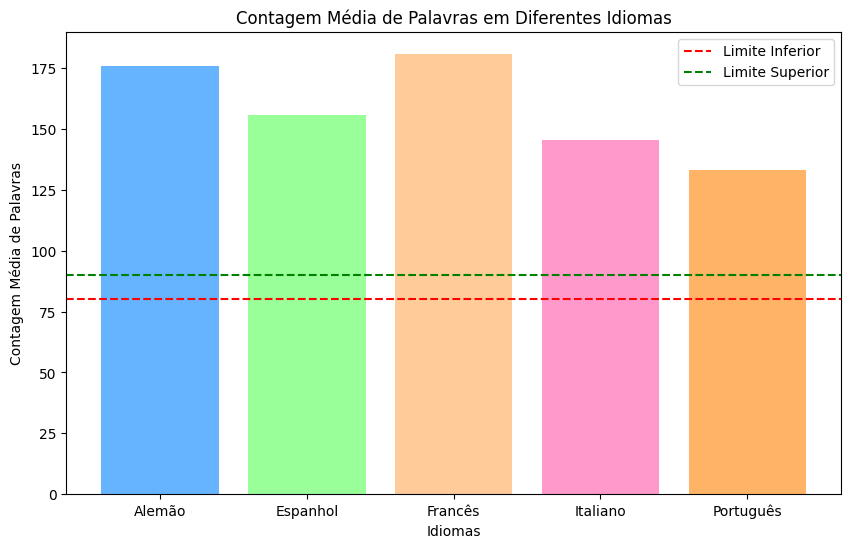
\includegraphics[width=\textwidth]{Fig1.png}
 \caption{Média de palavras nas línguas e níveis de proficiência: Nível A1.}
 \label{fig1}
 \source{Os autores.}
 \end{minipage}%
 \qquad
 \begin{minipage}{0.47\textwidth}
 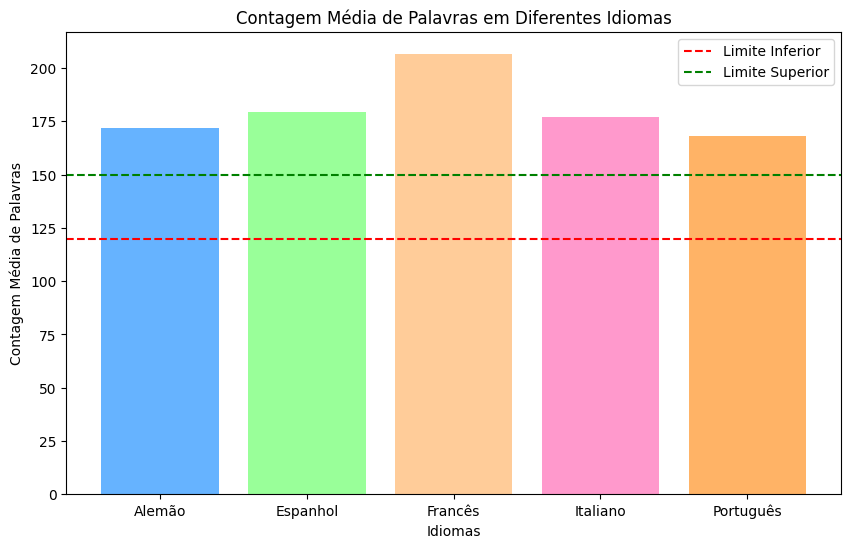
\includegraphics[width=\textwidth]{Fig2.png}
 \caption{Média de palavras nas línguas e níveis de proficiência: Nível A2.}
 \label{fig2}
 \source{Os autores.}
 \end{minipage}%
\end{figure}

\begin{figure}[p]
 \centering
 \begin{minipage}{.47\textwidth}
 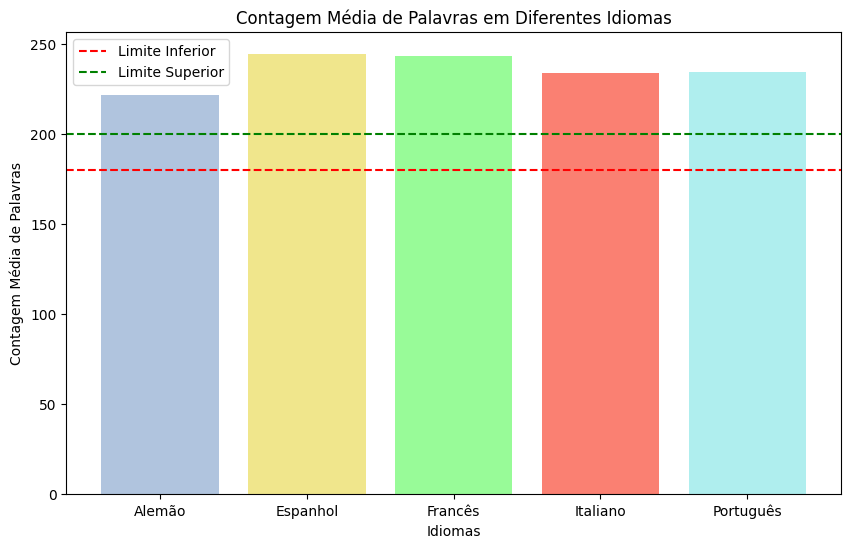
\includegraphics[width=\textwidth]{Fig3.png}
 \caption{Média de palavras nas línguas e níveis de proficiência: Nível B1.}
 \label{fig3}
 \source{Os autores.}
 \end{minipage}%
 \qquad
 \begin{minipage}{0.47\textwidth}
 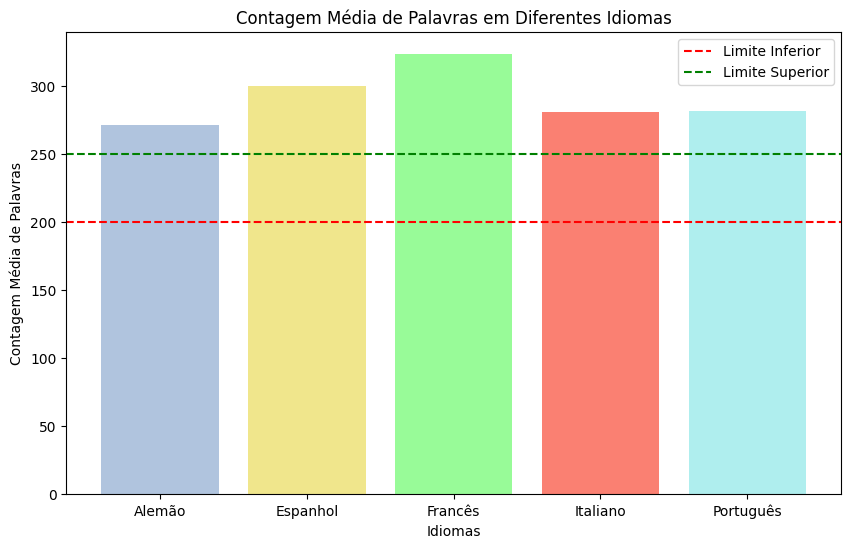
\includegraphics[width=\textwidth]{Fig4.png}
 \caption{Média de palavras nas línguas e níveis de proficiência: Nível B2.}
 \label{fig4} 
 \source{Os autores.}
 \end{minipage}%
\end{figure}

\begin{figure}[p]
 \centering
 \begin{minipage}{.47\textwidth}
 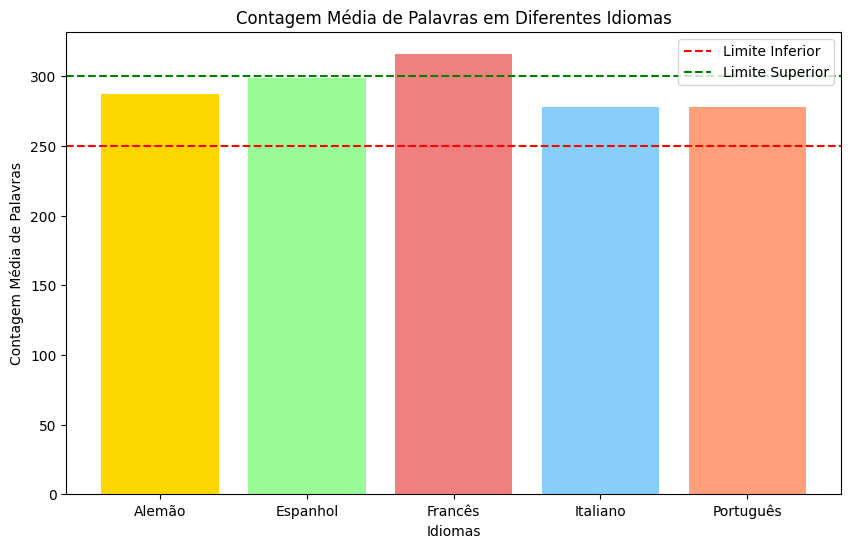
\includegraphics[width=\textwidth]{Fig5.png}
 \caption{Média de palavras nas línguas e níveis de proficiência: Nível C1.}
 \label{fig5}
 \source{Os autores.}
 \end{minipage}%
 \qquad
 \begin{minipage}{0.47\textwidth}
 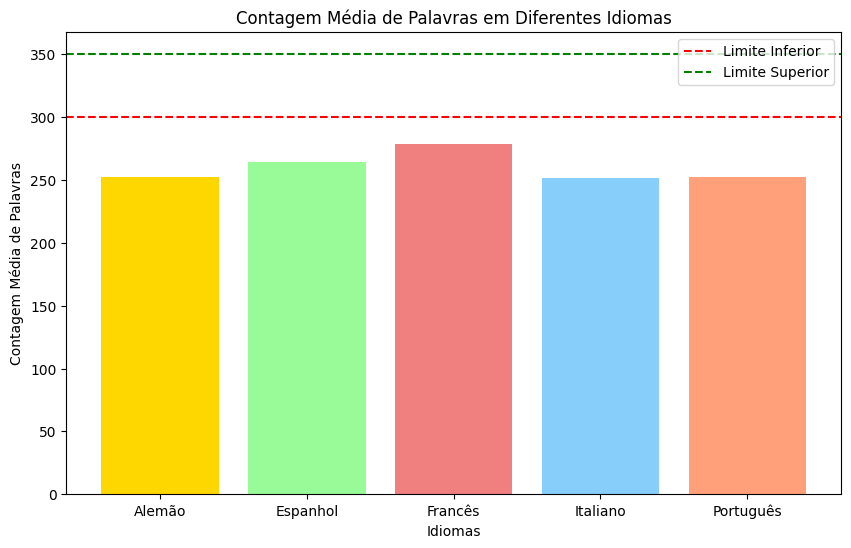
\includegraphics[width=\textwidth]{Fig6.png}
 \caption{Média de palavras nas línguas e níveis de proficiência: Nível C2.}
 \label{fig6} 
 \source{Os autores.}
 \end{minipage}%
\end{figure}

Os resultados mostram que a ferramenta de IA não segue as orientações das tarefas e sugerem uma tendência inversa ao que se esperaria de textos requeridos em níveis mais avançados de proficiência. Para os níveis iniciais, a ferramenta excede o número de palavras solicitadas e, inversamente, para os níveis finais, produz textos com número de palavras aquém do previsto.

A diferença de proporcionalidade no produto final do texto pode ser mais bem visualizada nas \Cref{tab02,tab03} subsequentes. A \Cref{tab02} mostra que o percentual de textos com número acima do solicitado se concentra nos níveis iniciais. 

\begin{table}[h!]
\centering
\begin{threeparttable}
\caption{Percentual de textos com palavras acima do esperado.}
\label{tab02}
\begin{tabular}{l l l l l l l}
\toprule
& Nível A1 & Nível A2 & Nível B1 & Nível B2 & Nível C1 & Nível C2 \\
 \midrule
Alemão & 99\% & 84\% & 83\% & 78\% & 33\% & 0\% \\
Espanhol  & 95\% & 88\% & 97\% & 88\% & 45\% & 3\% \\
Francês & 100\% & 98\% & 99\% & 99\% & 63\% & 1\% \\
Italiano & 94\% & 73\% & 89\% & 83\% & 19\% & 0\% \\
Português &  89\% & 76\% & 96\% & 86\% & 21\% & 0\% \\
\bottomrule
\end{tabular}
\source{Os autores.}
\end{threeparttable}
\end{table}

A tendência da ferramenta de IA foi de produzir os textos solicitados sem contemplar todos os aspectos das instruções inseridas no espaço previsto em sua plataforma. Esse resultado é reiterado nos dados apresentados na \Cref{tab03}, observando-os de outra perspectiva, ou seja, o número de palavras aquém do solicitado se concentra nos níveis finais. Confirma-se, assim, a tendência de não seguir todas as instruções solicitadas.

\begin{table}[h!]
\centering
\begin{threeparttable}
\caption{Percentual de textos com palavras abaixo do esperado.}
\label{tab03}
\begin{tabular}{l l l l l l l}
\toprule
& Nível A1 & Nível A2 & Nível B1 & Nível B2 & Nível C1 & Nível C2 \\
 \midrule
Alemão & 0\% & 0\% & 1\% & 0\% & 7\% & 96\% \\
Espanhol  &  2\% & 0\% & 0\% & 1\% & 3\% & 82\% \\
Francês & 0\% & 0\% & 0\% & 0\% & 0\% & 72\% \\
Italiano & 1\% & 3\% & 1\% & 0\% & 16\% & 90\% \\
Português & 0\% & 1\% & 0\% & 0\% & 19\% & 93\% \\
\bottomrule
\end{tabular}
\source{Os autores.}
\end{threeparttable}
\end{table}

Olhando os dois movimentos apresentados pelo ChatGPT conjuntamente, desde o ponto de vista do percentual de textos com número de palavras aquém do esperado e acima do solicitado, respectivamente, a \Cref{fig7} ilustra claramente esse produto textual e revela um movimento inverso, se comparados os níveis iniciais e finais. 

\begin{figure}[h!]
    \centering
    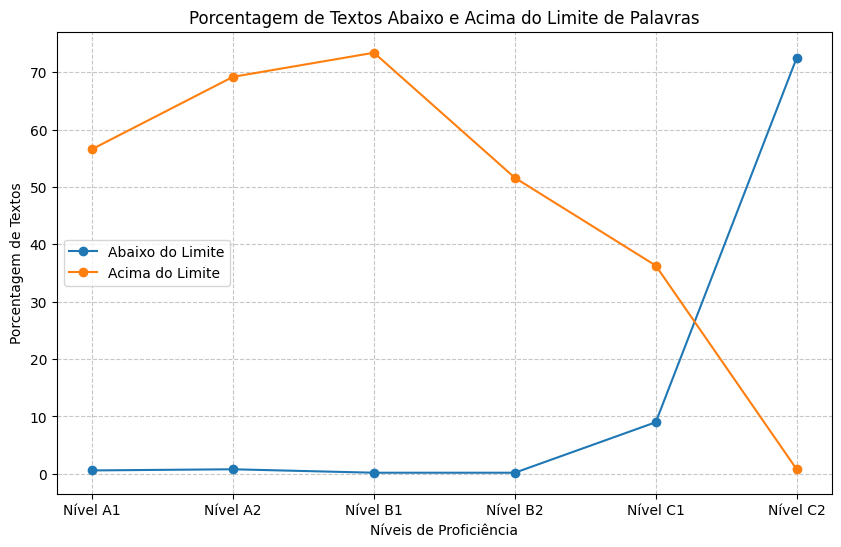
\includegraphics[width=0.8\linewidth]{Fig7.png}
    \caption{Percentual de textos com número de palavras distinto do esperado}
    \label{fig7}
    \source{Os autores.}
\end{figure}


Considerando-se as línguas adicionais contempladas neste estudo, selecionou-se uma segunda pergunta orientadora na análise dos dados, qual seja: \textit{O ChatGPT produz dados que revelam densidade lexical distinta entre as línguas adicionais e níveis de proficiência?}. Sistematizaram-se os resultados na \Cref{tab04}. 

\begin{table}[h!]
\centering
\begin{threeparttable}
\caption{Densidade lexical por línguas e níveis.}
\label{tab04}
\begin{tabular}{l l l l l l l}
\toprule
& Nível A1 & Nível A2 & Nível B1 & Nível B2 & Nível C1 & Nível C2 \\
 \midrule
Alemão & 41.57 & 44.16 & 37.74 & 45.14 & 40.64 & 43.89 \\
Espanhol  & 48.00 & 50.67 & 44.03 & 46.91 & 44.45 & 47.45 \\
Francês & 42.67 & 48.18 & 47.28 & 48.38 & 43.28 & 48.09 \\
Italiano & 46.51 & 49.51 & 49.47 & 49.53 & 45.05 & 48.78 \\
Português & 50.83 & 54.31 & 46.00 & 50.96 & 47.71 & 50.63 \\
\bottomrule
\end{tabular}
\source{Os autores.}
\end{threeparttable}
\end{table}


Para melhor visualizar os resultados em termos percentuais, a \Cref{fig8} ilustra esse comportamento revelado pela IA na produção escrita.

\begin{figure}[h!]
    \centering
    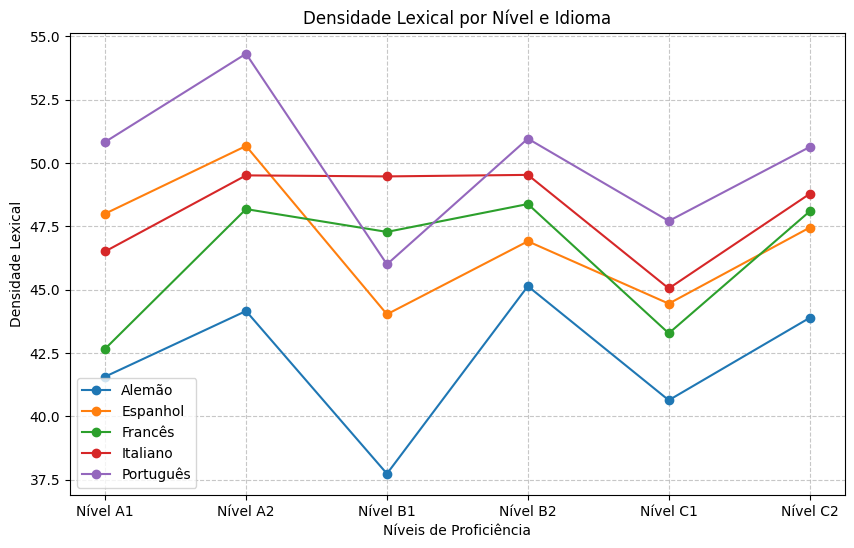
\includegraphics[width=0.8\linewidth]{Fig8.png}
    \caption{Densidade lexical por nível e idioma.}
    \label{fig8}
    \source{Os autores.}
\end{figure}

Os resultados na \Cref{fig8} sugerem uma tendência semelhante no movimento da densidade lexical em todas as línguas e níveis. Porém, os textos do nível A2 apresentaram densidade lexical mais alta do que se espera para este nível, contrariando a literatura da área a qual indica que esse percentual de densidade representaria a escrita de textos em níveis mais avançados de proficiência \cite{gregori-signes_analysing_2015,clavel-arroitia_analysing_2021}. A exceção foi para os dados no alemão para o nível B2, que apresentou percentual um pouco mais alto. Um segundo aspecto é a queda brusca no nível B1 do alemão, indicando uma diferença entre as línguas, e essa tendência se verifica também em espanhol e português. Portanto, os resultados permitem que se afirme haver diferenças nesse nível entre as línguas, conforme indicado pelo texto gerado para o nível B1, embora para duas línguas haja um movimento mais estável entre os níveis A2 e B2 (italiano e francês). Por outro lado, há uma semelhança entre as línguas com relação ao percentual, sugerindo que a ferramenta parece optar por certa formalidade do texto escrito. Esse resultado é corroborado no estudo de \textcite{gonzalez_fernandez_big_2018}, que analisou um corpus usando mensagens escritas no Twitter e destacou que a densidade lexical varia em um \textit{continuum} entre oralidade e escrita, sendo mais baixa quando o texto possui marcas de oralidade. 

Ao observar os resultados em uma mesma língua, ou seja, se \textit{o ChatGPT produz dados que revelam densidade lexical distinta em uma mesma língua considerando os níveis de proficiência}, os resultados ilustrados na \Cref{fig8} sugerem haver uma distinção em todas as línguas. Se comparadas as tarefas relativas ao nível A1 e C2, que se relacionam aos níveis de proficiência, a expectativa era de que haveria um percentual mais alto no C2; no entanto, não foi o que se concretizou nos dados, e os resultados confirmam que a ferramenta não consegue perceber esses detalhes do ponto de vista linguístico.

Por fim, para entender melhor os resultados, procedeu-se à análise orientada pela quarta pergunta de pesquisa: \textit{o ChatGPT produz dados que demonstram correlação entre a densidade lexical e a extensão textual em cada nível de proficiência?} Para responder a esta pergunta, recorreu-se a uma análise estatística usando o SPSS. Devido à quantidade de textos, 2991, e à natureza da análise, estes foram agrupados de acordo com os níveis do CEFR (498 textos no nível A1, 500 textos no nível A2, 500 textos no nível B1, 497 textos no nível B2, 498 textos no nível C1, e 498 textos no nível C2, respectivamente), visando a um tratamento estatístico mais significativo. A hipótese inicial é que a densidade aumentaria proporcionalmente aos níveis de proficiência e ao número de palavras. Para tanto, foram utilizados dados para contemplar duas variáveis que respondem a esta pergunta de pesquisa: qual é a densidade lexical e o número total de palavras de cada texto? Ambas as variáveis foram calculadas por meio do uso do Python nos ambientes Google Colab e Jupyter notebook e em planilhas de Excel antes de serem submetidas a uma análise detalhada em SPSS.

No SPSS, adotaram-se duas funções para analisar a correlação entre a extensão textual e a densidade lexical: a \textit{correlação bivariada} e a \textit{regressão linear}, a qual se subdivide em quatro itens de análise: variáveis inseridas/removidas, resumo do modelo, ANOVA e coeficientes. Dentre os resultados derivados dessa análise detalhada, três coeficientes são significativos para este estudo e serão discutidos a seguir: coeficiente de correlação, coeficiente valor de t (\textit{t-value})/Constante e o coeficiente valor de t (\textit{t-value})/\textit{TotaldePalavras}. A \Cref{tab05} elenca os resultados dos três coeficientes de acordo com cada nível do CEFR.

\begin{table}[h!]
\centering
\begin{threeparttable}
\caption{Resumo dos Coeficientes por nível.}
\label{tab05}
\begin{tabular}{p{2.0cm} p{3.0cm} p{4.0cm} p{4.0cm}}
\toprule
& Coeficiente de correlação & Coeficiente valor de t (t-value) - Constante & Coeficiente valor de t (t-value) - TotaldePalavras \\
 \midrule
Nível A1 & -0.544 & < 0.001 & < 0.001 \\
Nível A2 & -0.142 & < 0.001 & 0.001 \\
Nível B1 & 0.124 & < 0.001 & 0.006 \\
Nível B2 & 0.011 & < 0.001 & 0.808 \\
Nível C1 & -0.179 & < 0.001 & < 0.001 \\
Nível C2 & -0.039 & < 0.001 & 0.389 \\
\bottomrule
\end{tabular}
\source{Os autores.}
\end{threeparttable}
\end{table}

Os valores são também visualizados na \Cref{fig9}.

\begin{figure}[h!]
    \centering
    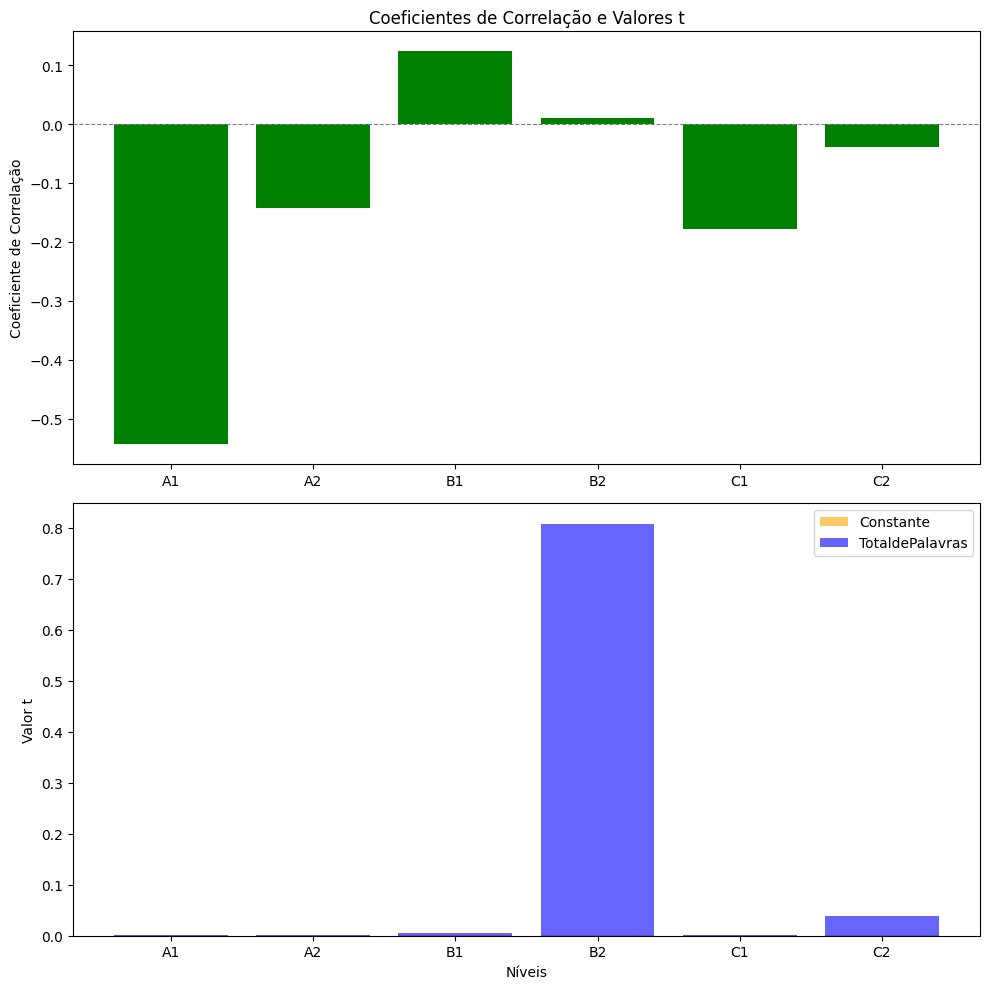
\includegraphics[width=0.8\linewidth]{Fig9.png}
    \caption{Coeficientes de Correlação e Valores de t (t-value).}
    \label{fig9}
    \source{Os autores.}
\end{figure}

Os resultados dos coeficientes em cada nível permitem estabelecer se há uma correlação entre o número de palavras e a densidade lexical. Para cada nível, são mostrados os resultados sob o formato de Tabelas seriadas no SPSS. Primeiro, o foco de análise é nas tabelas de \textit{Correlações} para entender o coeficiente de correlação nos seis níveis do CEFR e, em seguida, as tabelas de Coeficientes para explicar os coeficientes valor de t \textit{Constante} e \textit{TotaldePalavras}.

O coeficiente de correlação advém do primeiro passo da análise em SPSS, ilustrada na \Cref{fig10} do Nível A1 e detalhada a seguir. Procedimento similar foi aplicado aos demais níveis.

\begin{figure}[h!]
    \centering
    
\includegraphics[width=0.8\linewidth]{Fig10.png}
    \caption{Correlações Nível A1.}
    \label{fig10}
    \source{Os autores.}
\end{figure}

A verificação da existência de uma correlação entre o número total de palavras e a densidade lexical e seus elementos oferece diferentes informações: a correlação de Pearson (\textit{Pearson’s r}) estabelece a correlação entre as duas variáveis \textit{DensidadeLexical} e \textit{TotaldePalavras}, a qual é de –0.544 nesse caso, e quantifica a força e a direção linear entre as duas variáveis. Essa correlação negativa indica que, à medida que o número de palavras aumenta, a densidade lexical diminui, e vice-versa. No que concerne ao Nível de Significância (\textit{Sig.}), o valor de p (\textit{p-value}), nesse caso < 0,001, indica a probabilidade de a correlação entre as duas variáveis ter ocorrido por acaso ou não. No presente caso, é improvável ter sido por acaso e, portanto, é considerada significativa. Por último, o elemento N indica o tamanho da amostra (498 textos).

No nível A1, os resultados sugerem uma correlação negativa forte entre o número total de palavras em um texto e sua densidade lexical, e essa relação é estatisticamente significativa. À medida que os textos se tornam mais longos (com mais palavras), eles tendem a ter uma densidade lexical menor e, inversamente, textos mais curtos tendem a ter uma densidade lexical maior. Isso poderia implicar que textos mais longos podem incluir palavras redundantes ou menos informativas, levando a uma densidade lexical menor. Entretanto, isso demandaria uma análise qualitativa que não está no escopo deste estudo.

No nível A2, os resultados (cf. \Cref{fig11}) mostram que o coeficiente da correlação de Pearson entre as duas variáveis é aproximadamente –0.142, o que sugere uma correlação negativa fraca entre as duas variáveis. Como ocorreu com os textos no nível A1, à medida que o número de palavras no texto aumenta, a densidade lexical tende a diminuir, e vice-versa. A correlação é significativa no nível 0,01 (2 extremidades) e indica que a correlação é significante estatisticamente em um alto nível de confiança e não ocorreu por acaso. No entanto, é importante frisar que, apesar de ser estatisticamente significativa, a força da correlação entre as duas variáveis é relativamente fraca.

\begin{figure}[h!]
    \centering
    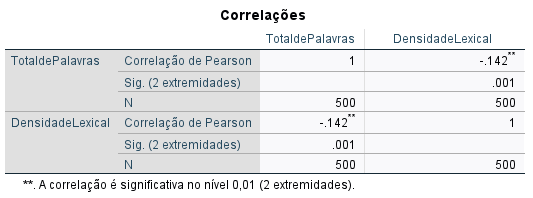
\includegraphics[width=0.8\linewidth]{Fig11.png}
    \caption{Correlações Nível A2.}
    \label{fig11}
    \source{Os autores.}
\end{figure}

No nível B1, evidenciados pela \Cref{fig12}, o coeficiente de correlação de Pearson é aproximadamente 0,124. Como ocorreu nos níveis A1 e A2, a correlação é considerada estatisticamente significativa no nível de significância de 0,01 (bilateral), ou seja, é improvável de ter ocorrido por acaso. O coeficiente de correlação 0,124 sugere uma correlação positiva fraca entre as variáveis \textit{TotaldePalavras} e \textit{DensidadeLexical} e indica que, conforme o número total de palavras em um texto aumenta, a densidade lexical tende a aumentar ligeiramente, e vice-versa, diferente do que ocorreu nos níveis A1 e A2, respectivamente. No entanto, é importante salientar que, embora estatisticamente significativa, a força da correlação é relativamente fraca e sugere que outros fatores também podem influenciar a relação entre essas variáveis, como enfatizado anteriormente sobre o possível uso de palavras redundantes ou menos informativas.

\begin{figure}[h!]
    \centering
    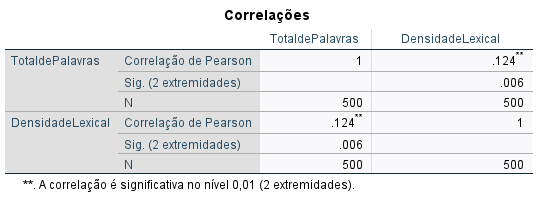
\includegraphics[width=0.8\linewidth]{Fig12.png}
    \caption{Correlações Nível B1.}
    \label{fig12}
    \source{Os autores.}
\end{figure}

Os resultados evidenciados na \Cref{fig13}, do nível B2, indicam que o coeficiente de correlação entre as duas variáveis é de aproximadamente 0,011, o que sugere uma correlação positiva muito fraca. Isso quer dizer que praticamente não há relação linear entre essas variáveis. Ademais, o valor de significância (\textit{Sig.}) elevado, 0,808, indica que a correlação observada não é estatisticamente significativa de acordo com os níveis de significância convencionais (por exemplo, $\alpha$ = 0,05). Ou seja, diferente dos níveis anteriores, a correlação entre as duas variáveis provavelmente se deve ao acaso e não possui significado prático ou relevante estatisticamente para este estudo.

\begin{figure}[h!]
    \centering
    
\includegraphics[width=0.8\linewidth]{Fig13.png}
    \caption{Correlações Nível B2.}
    \label{fig13}
    \source{Os autores.}
\end{figure}

No nível C1, a correlação entre as variáveis \textit{TotaldePalavras} e \textit{DensidadeLexical} é estatisticamente significativa no nível de 0,01 (duas extremidades), sugerindo que há um alto grau de confiança no resultado (\Cref{fig14}). O coeficiente de correlação é de aproximadamente -0,179 e indica haver uma correlação negativa moderada entre as duas variáveis. Isso quer dizer que, à medida que o total de palavras em um texto aumenta, a densidade lexical tende a diminuir e o sinal negativo do coeficiente transparece uma relação inversa entre as variáveis. O baixo valor de p (\textit{Sig.}), menor que 0,001, prediz que é bastante improvável que a correlação observada tenha ocorrido por acaso e é, portanto, relevante para este estudo.  

\begin{figure}[h!]
    \centering
    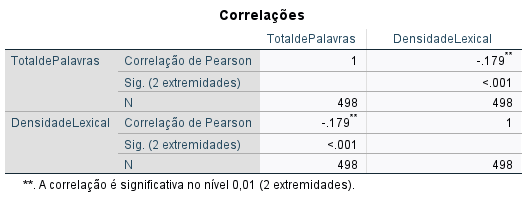
\includegraphics[width=0.8\linewidth]{Fig14.png}
    \caption{Correlações Nível C1.}
    \label{fig14}
    \source{Os autores.}
\end{figure}

Por último, no nível C2 (\Cref{fig15}), os resultados indicam que o coeficiente de correlação entre as variáveis \textit{TotaldePalavras} e \textit{DensidadeLexical} é -0.039, sugerindo haver uma correlação negativa muito fraca, ou seja, há pouca ou nenhuma relação linear entre essas duas variáveis. O valor de p (0,389) é considerado relativamente alto, externando que a correlação poderia ser explicada razoavelmente pelo acaso, mas que a mesma não é estatisticamente significativa. Portanto, no nível C2, assim como ocorreu em B2, parece não haver uma correlação significativa ou relevante entre as duas variáveis.

\begin{figure}[h!]
    \centering
    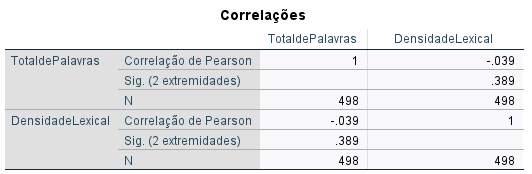
\includegraphics[width=0.8\linewidth]{Fig15.png}
    \caption{Correlações Nível C2.}
    \label{fig15}
    \source{Os autores.}
\end{figure}

Para confirmar a análise inicialmente feita usando a função correlação, o segundo passo foi usar a função regressão linear. Dentre as subdivisões desta função, é trazida para esta discussão a chamada Coeficientes, a qual se subdivide em dois coeficientes distintos: valor de t (\textit{t-value})/Constante e coeficiente valor de t (\textit{t-value})/\textit{TotaldePalavras}. A mesma análise foi conduzida em todos os níveis e é ilustrada na \Cref{fig16}, utilizando o resultado do nível A1.

\begin{figure}[h!]
    \centering
    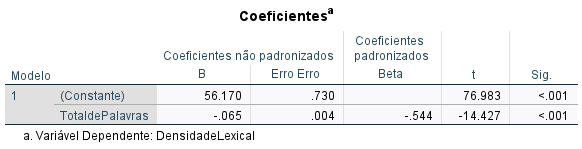
\includegraphics[width=0.8\linewidth]{Fig16.png}
    \caption{Coeficientes Nível A1.}
    \label{fig16}
    \source{Os autores.}
\end{figure}

A Tabela \textit{Coeficientes} contém informações sobre os coeficientes do modelo de regressão, os quais ajudam, neste estudo, a compreender as relações entre as chamadas \textit{variável preditora} (\textit{TotaldePalavras}) e a \textit{variável dependente} (\textit{DensidadeLexical}). O coeficiente padronizado (Beta) destaca a importância relativa de cada variável preditora na explicação da variabilidade na variável dependente. O valor de t indica quantos erros padrão o coeficiente está afastado de zero, e o coeficiente padronizado oferece uma ideia do tamanho do efeito em termos de desvio padrão. Ambos o \textit{valor de t} e o \textit{valor de significância} (\textit{Sig.}) assinalam a significância estatística de cada coeficiente.

No que diz respeito à regressão no Nível A1, portanto, o coeficiente negativo para a variável preditora \textit{TotaldePalavras} sugere que, à medida que o número total de palavras em um texto aumenta, a densidade lexical tende a diminuir. Ambos os coeficientes são estatisticamente significativos (<0,001), mostrando que as relações dificilmente ocorreram por acaso. Assim, esses resultados confirmam aqueles obtidos na análise do coeficiente de correlação na primeira parte da análise. O mesmo ocorre no Nível A2 (\Cref{fig17}), em que o coeficiente negativo para a variável preditora \textit{TotaldePalavras} também confirma que, à medida que o número total de palavras de um texto aumenta, a densidade lexical tende a diminuir ligeiramente. Ambos os coeficientes são estatisticamente significativos (p < 0,001 para \textit{Constante} e p = 0,001 para \textit{TotaldePalavras}) e sinalizam que as relações dificilmente ocorreram por acaso. 

\begin{figure}[h!]
    \centering
    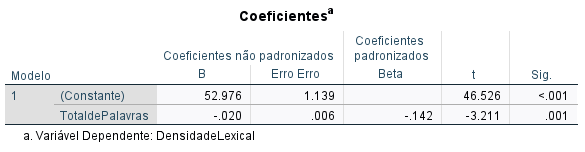
\includegraphics[width=0.8\linewidth]{Fig17.png}
    \caption{Coeficientes Nível A2.}
    \label{fig17}
    \source{Os autores.}
\end{figure}

Os resultados obtidos no Nível B1 (\Cref{fig18}) também corroboram os obtidos pelo cálculo do coeficiente de correlação na primeira parte da análise. O coeficiente positivo para a variável preditora \textit{TotaldePalavras} indica que, à medida que o número total de palavras em um texto aumenta, a densidade lexical tende a aumentar ligeiramente. Ambos os coeficientes são estatisticamente significativos (p < 0,001 para \textit{Constante} e p = 0,006 para \textit{TotaldePalavras}), preconizando que as relações dificilmente ocorreram por acaso.

\begin{figure}[h!]
    \centering
    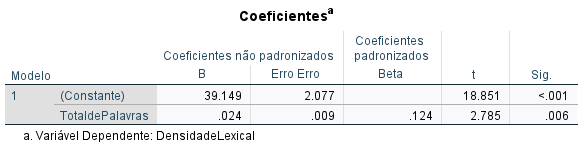
\includegraphics[width=0.8\linewidth]{Fig18.png}
    \caption{Coeficientes Nível B1.}
    \label{fig18}
    \source{Os autores.}
\end{figure}

Já no Nível B2 (\Cref{fig19}), o coeficiente positivo para a variável preditora \textit{TotaldePalavras} denota haver uma associação positiva entre o número total de palavras e a densidade lexical, mas o efeito é extremamente pequeno. Já o valor de p não significativo (0,808) para a variável preditora \textit{TotaldePalavras} revela que a relação entre esse preditor e a variável dependente não é estatisticamente significativa, confirmando o que foi sugerido pela análise do coeficiente de correlação na primeira parte da análise.

\begin{figure}[h!]
    \centering
    
\includegraphics[width=0.8\linewidth]{Fig19.png}
    \caption{Coeficientes Nível B2.}
    \label{fig19}
    \source{Os autores.}
\end{figure}

No nível C1 (\Cref{fig20}), o coeficiente negativo para a variável preditora \textit{TotaldePalavras} sinaliza haver uma associação negativa entre o número total de palavras e a densidade lexical. Ou seja, à medida que o número de palavras de um texto aumenta, a densidade lexical tende a diminuir, corroborando o que foi verificado na análise do coeficiente de correlação na primeira parte da análise. O alto valor absoluto de t (\textit{t-value}) (-4,045) e o valor de p muito baixo (menor que 0,001) para a variável preditora \textit{TotaldePalavras} indicam que a relação entre esta e a variável dependente é estatisticamente significativa. 

\begin{figure}[h!]
    \centering
    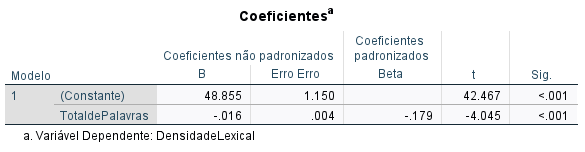
\includegraphics[width=0.8\linewidth]{Fig20.png}
    \caption{Coeficientes Nível C1.}
    \label{fig20}
    \source{Os autores.}
\end{figure}

Por fim, no nível C2 (\Cref{fig21}), o valor de t (t-value) e o valor associado de p oferecem informação sobre a significância estatística da variável preditora \textit{TotaldePalavras}. Nesse caso, o valor de p para \textit{TotaldePalavras}, 0,389, é considerado relativamente alto e sugere que a relação entre as duas variáveis pode não ser estatisticamente significativa e, portanto, confirma o resultado da análise do coeficiente de correlação. Ademais, o baixo coeficiente padronizado (Beta) (-0.039) e o alto valor de p sugerem que a variável preditora não parece ter um impacto substancial na variável dependente. 

\begin{figure}[h!]
    \centering
    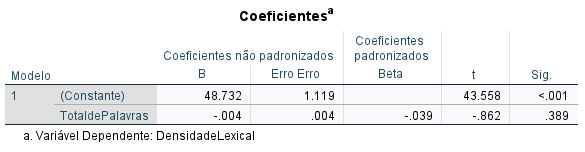
\includegraphics[width=0.8\linewidth]{Fig21.png}
    \caption{Coeficientes Nível C2.}
    \label{fig21}
    \source{Os autores.}
\end{figure}

Apresentados os dados e indicados os resultados, orientados pelas perguntas de pesquisa, na próxima seção são discutidos esses resultados e indicadas as contribuições deste estudo.

\section{Discussão e considerações finais}\label{sec-formato}
Este estudo discutiu a escrita em línguas adicionais para compreender o impacto que as ferramentas digitais exercem na produção textual. Para tanto, analisou a densidade lexical na perspectiva da LSF \cite{halliday_spoken_1985,halliday_grammatical_1993} em um \textit{corpus} resultante de seis tarefas produzidas pelo ChatGPT em cinco idiomas (alemão, espanhol, francês, italiano e português) e comparou a densidade lexical entre essas línguas e níveis de proficiência para identificar se haveria um padrão que indicasse complexidade textual. 

A análise foi sistematizada em tabelas e figuras para visualizar os resultados, considerando-se as línguas adicionais e respectivos níveis de proficiência. Evidenciaram-se os valores da densidade lexical em cada língua (cf. \Cref{fig1,fig2,fig3,fig4,fig5,fig6} e \Cref{tab02,tab03}), para verificar o quão consistentes foram esses valores. 

Com relação à primeira pergunta de pesquisa (cf. \Cref{fig1,fig2,fig3,fig4,fig5,fig6}, \Cref{tab02,tab03} e \Cref{fig7}), os resultados mostraram que a ferramenta de IA não é sensível às especificidades das orientações indicadas para a realização da tarefa nem à variável proficiência. O ChatGPT produziu textos com extensão diversa ao solicitado, não considerando os níveis de proficiência indicados. Portanto, é um resultado incongruente ao esperado na produção de textos em uma língua adicional por humanos. 

Os resultados relativos às segunda e terceira perguntas deste estudo mostraram que o ChatGPT produziu dados que seguem um mesmo padrão, independente da língua adicional. Esse padrão foi verificado na extensão dos textos; no entanto, entre os níveis de proficiência, observou-se uma diferença para os textos do nível B1. Esse padrão é reiterado quando se verifica o que acontece em uma mesma língua e níveis de proficiência. Em outras palavras, independente da língua adicional, o ChatGPT não produz textos que revelam diferenças marcantes entre os níveis iniciais e finais, respectivamente.

Para reforçar os resultados revelados pelos dados estatísticos, análises de correlações e coeficientes foram realizadas com o propósito de verificar se o “\textit{ChatGPT produz dados que demonstram correlação entre a densidade lexical e a extensão textual em cada nível de proficiência}” (4a. pergunta de pesquisa). Os resultados dos coeficientes revelaram a seguinte correlação entre o número de palavras e a densidade lexical: para o nível A1, uma não correlação negativa forte; para o nível A2, negativa fraca; para o nível B1, correlação positiva fraca, diferenciando-se dos dois níveis anteriores e confirmando a diferença observada em termos de percentuais de densidade lexical. Por sua vez, no nível B2, verificou-se uma correlação positiva muito fraca; no nível C1, correlação negativa moderada; no nível C2, correlação negativa muito forte. 

Para a confirmação desses resultados, empreendeu-se uma análise utilizando a função regressão linear. Os resultados mostraram coeficiente negativo para o coeficiente de valor t (\textit{t-value}), \textit{TotaldePalavras} no nível A1, reiterando a análise anterior; o nível A2 revelou coeficiente negativo de valor t (\textit{t-value})/\textit{TotaldePalavras}; o nível B1 confirmou o resultado indicado na \Cref{fig12}, cujos coeficientes são estatisticamente positivos para o valor de t (\textit{t-value})/\textit{TotaldePalavras}; o nível B2 revelou coeficiente positivo, associação positiva entre as variáveis; o nível C1 mostrou coeficiente negativo para a variável preditora \textit{TotaldePalavras} com associação negativa entre o número total de palavras e a densidade lexical. Finalmente, o nível C2 exibiu significância relativamente alta, confirmando o que foi sugerido na análise do coeficiente de correlação.

Portanto, os resultados permitem que se conclua que, a partir da comparação entre as diferentes línguas adicionais, a ferramenta de IA não é sensível às características do sistema linguístico como, por exemplo, línguas adicionais mais desinenciais em relação às que não o são, pois as diferenças em termos percentuais são moderadas. Além disso, não se observou, com base nos padrões verificados, haver alguma língua, dentre as cinco, que revelasse um padrão muito diferente das demais. Por outro lado, levando-se em conta a variável nível de proficiência, obtiveram-se dois resultados inesperados: o nível A2, que se diferencia dos demais, e o nível C1, que apresenta um decréscimo quanto à densidade lexical em todas as línguas, resultado que difere daqueles que discutem proficiência linguística em contexto de língua adicional \cite{kondal_effects_2015,schnur_lexical_2021}.

Esses resultados divergem das observações feitas no estudo de \textcite{lancaster_artificial_2023}, que salienta que o ChatGPT responde de maneira pré-determinada com base em sua programação (ou modelo criado), visto que, se a mesma entrada for inserida, a tendência da ferramenta é dar as mesmas respostas. A divergência diz respeito ao fato de a ferramenta produzir textos com extensão distinta entre as línguas adicionais, níveis de proficiência e densidade lexical, embora as especificidades do sistema linguístico de cada língua poderiam ser determinantes. A esse respeito, os dados requereriam um tratamento qualitativo para cada um dos textos do \textit{corpus}. 

Os resultados também dão indicações de que a ferramenta precisa ser mais bem refinada para levar em conta as características linguísticas de cada língua adicional e produzir textos escritos que tenham dados confiáveis que possam revelar a proficiência linguística em uso e real se comparada à produção escrita sem auxílio da IA. Nesse sentido, o uso da ferramenta em contexto de ensino precisa acontecer com parcimônia. 

A contribuição deste estudo, a exemplo do que já sinalizou \textcite{lancaster_artificial_2023}, indica que o ChatGPT é parte do desenvolvimento tecnológico que precisa se coadunar com o desenvolvimento educacional para que estudantes ou usuários da ferramenta compreendam: o uso tem implicações éticas e limitações, não sendo uma solução mágica para produzir textos escritos; os vários campos do conhecimento possuem exigências diferentes, como é o caso do ensino de línguas adicionais e a proficiência escrita nessas línguas para não gerar dados imprecisos; a possibilidade de questionar informações. Por fim, quanto à densidade lexical, este artigo é pioneiro em abordar o tema nesse contexto, e a principal contribuição é compreender a complexidade dos textos que são produzidos por essa ferramenta. 

Futuras pesquisas são necessárias com textos produzidos pelo ChatGPT para compreender melhor a qualidade e a complexidade da escrita em termos da organização dos complexos oracionais, da complexidade sintática e modalidade e avaliatividade sob a perspectiva da LSF. Além disso, pesquisas que analisem os textos qualitativamente e relacionem a qualidade da escrita em termos de níveis de proficiência de acordo com o CEFR serão bem-vindas. Por fim, pesquisas que explicitem de que forma os textos produzidos pelo ChatGPT podem levantar questões pedagógicas e suas possíveis contribuições para o desenvolvimento do currículo no ensino de línguas adicionais são desejáveis. 



\section{Financiamento}\label{sec-conclusao}
A coleta de dados para o presente estudo foi financiada por meio do Executive Dean Fund da University of Essex, Reino Unido, e faz parte do projeto "The Effect of ChatGPT on Student Writing in Multiple Languages: A Systemic Functional Linguistics Analysis".


\printbibliography\label{sec-bib}
% if the text is not in Portuguese, it might be necessary to use the code below instead to print the correct ABNT abbreviations [s.n.], [s.l.]
%\begin{portuguese}
%\printbibliography[title={Bibliography}]
%\end{portuguese}


%full list: conceptualization,datacuration,formalanalysis,funding,investigation,methodology,projadm,resources,software,supervision,validation,visualization,writing,review
\begin{contributors}[sec-contributors]
\authorcontribution{Antonio Marcio da Silva}[conceptualization,formalanalysis,funding,methodology,resources,writing,review]
\authorcontribution{Lucia Rottava}[conceptualization,formalanalysis,methodology,resources,writing,review]
\end{contributors}

\appendix 
\section{Anexo}\label{apx-longtable}
Instruções das atividades realizadas pelos participantes

\begin{figure}[h!]
    \centering
    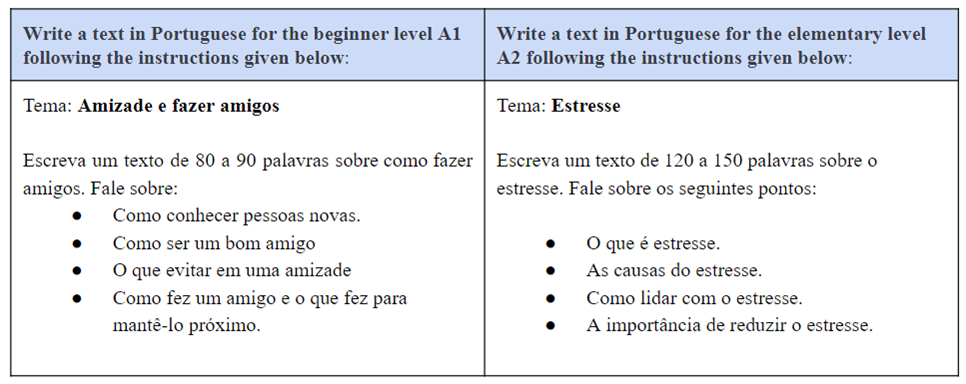
\includegraphics[width=0.8\linewidth]{Fig22.png}
    \label{fig22}
\end{figure}

\begin{figure}[h!]
    \centering
    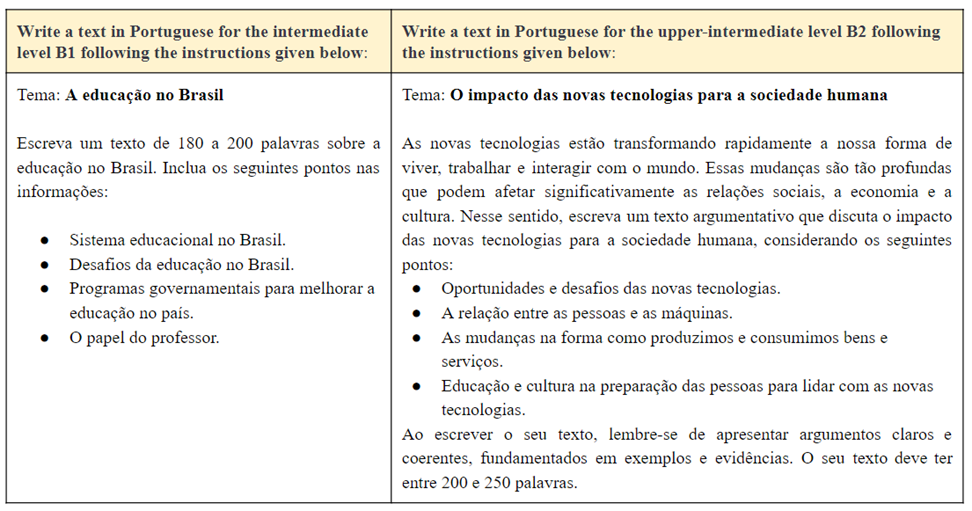
\includegraphics[width=0.8\linewidth]{Fig23.png}
    \label{fig23}
\end{figure}

\begin{figure}[h!]
    \centering
    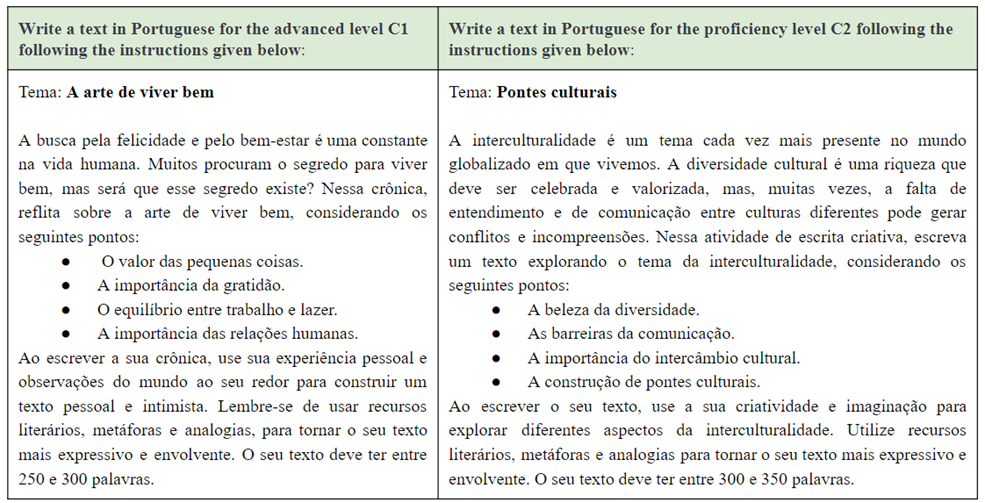
\includegraphics[width=0.8\linewidth]{Fig24.png}
    \label{fig24}
\end{figure}
\end{document}

